\renewcommand{\SS}{\mathbb{S}}
\newcommand{\Par}[2]{\mbox{$( #1, #2 )$}}
\usetikzlibrary{positioning, shapes, trees, graphs} % RNA trees
\newcommand{\scale}{0.6}

\newcommand{\tree}[1]{\ensuremath{#1}}

\chapter{Úvod do štúdia RNA štruktúry a grafov}

V tejto časti práce zoznámime čitateľa s pojmami, ktoré s RNA a jej
štruktúrou súvisia.

\section{Čo je RNA}

RNA, ribonukleová kyselina, je jednovláknová molekula, pozostávajúca
zo sekvencie nukleotidov, jej základných stavebných častí.
Tie sa ďalej skladajú z cukru (pentózy), dusíkatej bázy a zvyšku
kyseliny fosforečnej. Poznáme štyry druhy báz,
adenín, cytozín, guanín a uracyl, označovať ich budeme A, C, G, respektíve U.
Okrem báz nás ďalšie zložky nebudú zaujímať a tak ďalej v texte stotožníme
pojmy nukleotid a báza.

Štruktúru RNA môžeme chápať podľa stupňa zjednodušenia
\begin{itemize}
  \item Primárna štruktúra - poradie nukleotidov v reťazci
  \item Sekundárna štruktúra - párovanie medzi bázami
  \item Terciárna štruktúra - priestorové usporiadanie molekuly
\end{itemize}

RNA ako jednovláknová molekula sa v snahe minimalizovať voľnú energiu páruje sama na seba.
V tomto hrajú úlohu vodíkové väzby medzi nukleotidmi. Tie majú vzájomnú preferenciu,
čo znamená, že páry vznikajú najčastejšie medzi A-U a C-G, no ani iné
kombinácie nie sú vylúčené. 

\section{Sekundárna štruktúra}

Hlavným objektom nášho záujmu je sekundárna štruktúra RNA. V nasledujúcej
časti si ju definujeme formálnejšie.

\begin{definice}
  \label{def:RNA_primarna_struktura}
  Primárna štruktúra RNA je určená poradím nukleotidov v polynukleotidovom reťazci.
  \\
  Sekundárnou štruktúrou označíme množinu $\SS$ párov báz \Par{i}{j} takých,
  že pre dva páry \Par{i}{j} a \Par{k}{l} $\in \SS$ (bez straty na všeobecnosti $i \leq k$)
  platí jedno z nasledujúcich:
  \begin{itemize}
    \item $i = k \iff j = l$
    \item $i < j < k < l$, čiže pár \Par{i}{j} predchádza pár \Par{k}{l}
    \item $i < k < l < j$, čiže pár \Par{i}{j} obsahuje pár \Par{k}{l}
  \end{itemize}
\end{definice}

Prvá podmienka zabezpečuje, že nukleotid je najviac v jednom bázickom páre,
druhá a tretia hovoria o ich usporiadaní - buď na seba nadväzujú, alebo
sú na sebe nezávisle.

Všimnime si ďalej, že podmienky vylučujú bázové páry typu \Par{i}{j} a \Par{k}{l},
kde $i < k < j < l$, teda páry sa nesmú prekrývať. Takéto páry nazývame
pseudouzly (pseudoknot) a ich rozdelenie máme na obrázku \ref{obr:pseudoknot_types}.
Pseudouzly sa často považujú za súčasť sekundárnej štruktúry, no v našej práci
s nimi nepočítame. Takéto zjednodušenie nám umožní reprezentovať sekundárnu
štruktúru RNA ako usporiadaný zakorenený strom (les). Definíciu grafových
pojmov ako strom a les uvedieme neskôr.

\begin{figure}
%trim=left bottom right top
  \includegraphics[clip, trim=0 12cm 0 11cm, width=0.9\textwidth]{../img/pseudoknot}
  \caption{Typy pseudouzlov podľa \citenum{PSEUDOKNOT_TYPES}}
  \label{obr:pseudoknot_types}
\end{figure}

\section{Motívy}

Motivom v RNA máme na mysli časti molekuly, ktoré vytvárajú určité štruktúry.
Na obrazku \ref{obr:RNA_motifs} vidime motivy, ktore sa mozu v RNA vyskytovat.

Stem (stonka) je časť molekuly kde sa na seba paruju dva súvisle časti RNA vlákna.
Interior loop spája dva stemy a medzi nimi na oboch stranách obsahuje nespárované
bázy. Podobna je bulge (vypuklina), ale nespárované nukleotidy ma iba z jednej strany.
Hairpin je medzi časťami vlákna, ktoré sa parujú sami na seba.
Multibranch loop je podobná ako interior loop, ale spája dokopy viac stemov.
V ďalšom rozprávani ámam bude stačiť rozdelenie na stem a loop.

%TODO: ako nazyvat strukturne motivy v RNA: anglicky, alebo hladat vhodny preklad

\begin{figure}[H]
\centering
\includegraphics[width=70mm, height=70mm]{../img/struktury_v_rna.png}
\caption{Strukturalne motivy v RNA}
\label{obr:RNA_motifs}
\end{figure}


%TODO

\begin{figure}[H]
%TODO ostatne reprezentacie RNA
\centering
\includegraphics[width=140mm, height=120mm]{../img/RNA_circular_reprezentation.png}
\caption{Circular Feynman - kruhova reprezentacia sekundarnej struktury}
\label{obr:RNA_circular_representation}
\end{figure}

\section{Hlavný objekt záujmu - rRNA}

Ako hlavný objekt záujmu sme si spomedzi všetkych druhov RNA vybrali práve ribozomálnu, rRNA.
Jej funkcia je hlavne v translácií génov, pri ktorej sa genetická informácia prekladá
z poradia nukleotidov v mRNA do poradia aminokyselín v bielkovine.

\begin{figure}
  \includegraphics[width=1\textwidth]{../img/human_crw}
  \caption{Vizualizácia sekundárnej štruktúry RNA človeka z CRW databázy \citenum{CRW}}
  \label{obr:RNA_human_crw}
\end{figure}

\begin{figure}
%trim=left bottom right top
  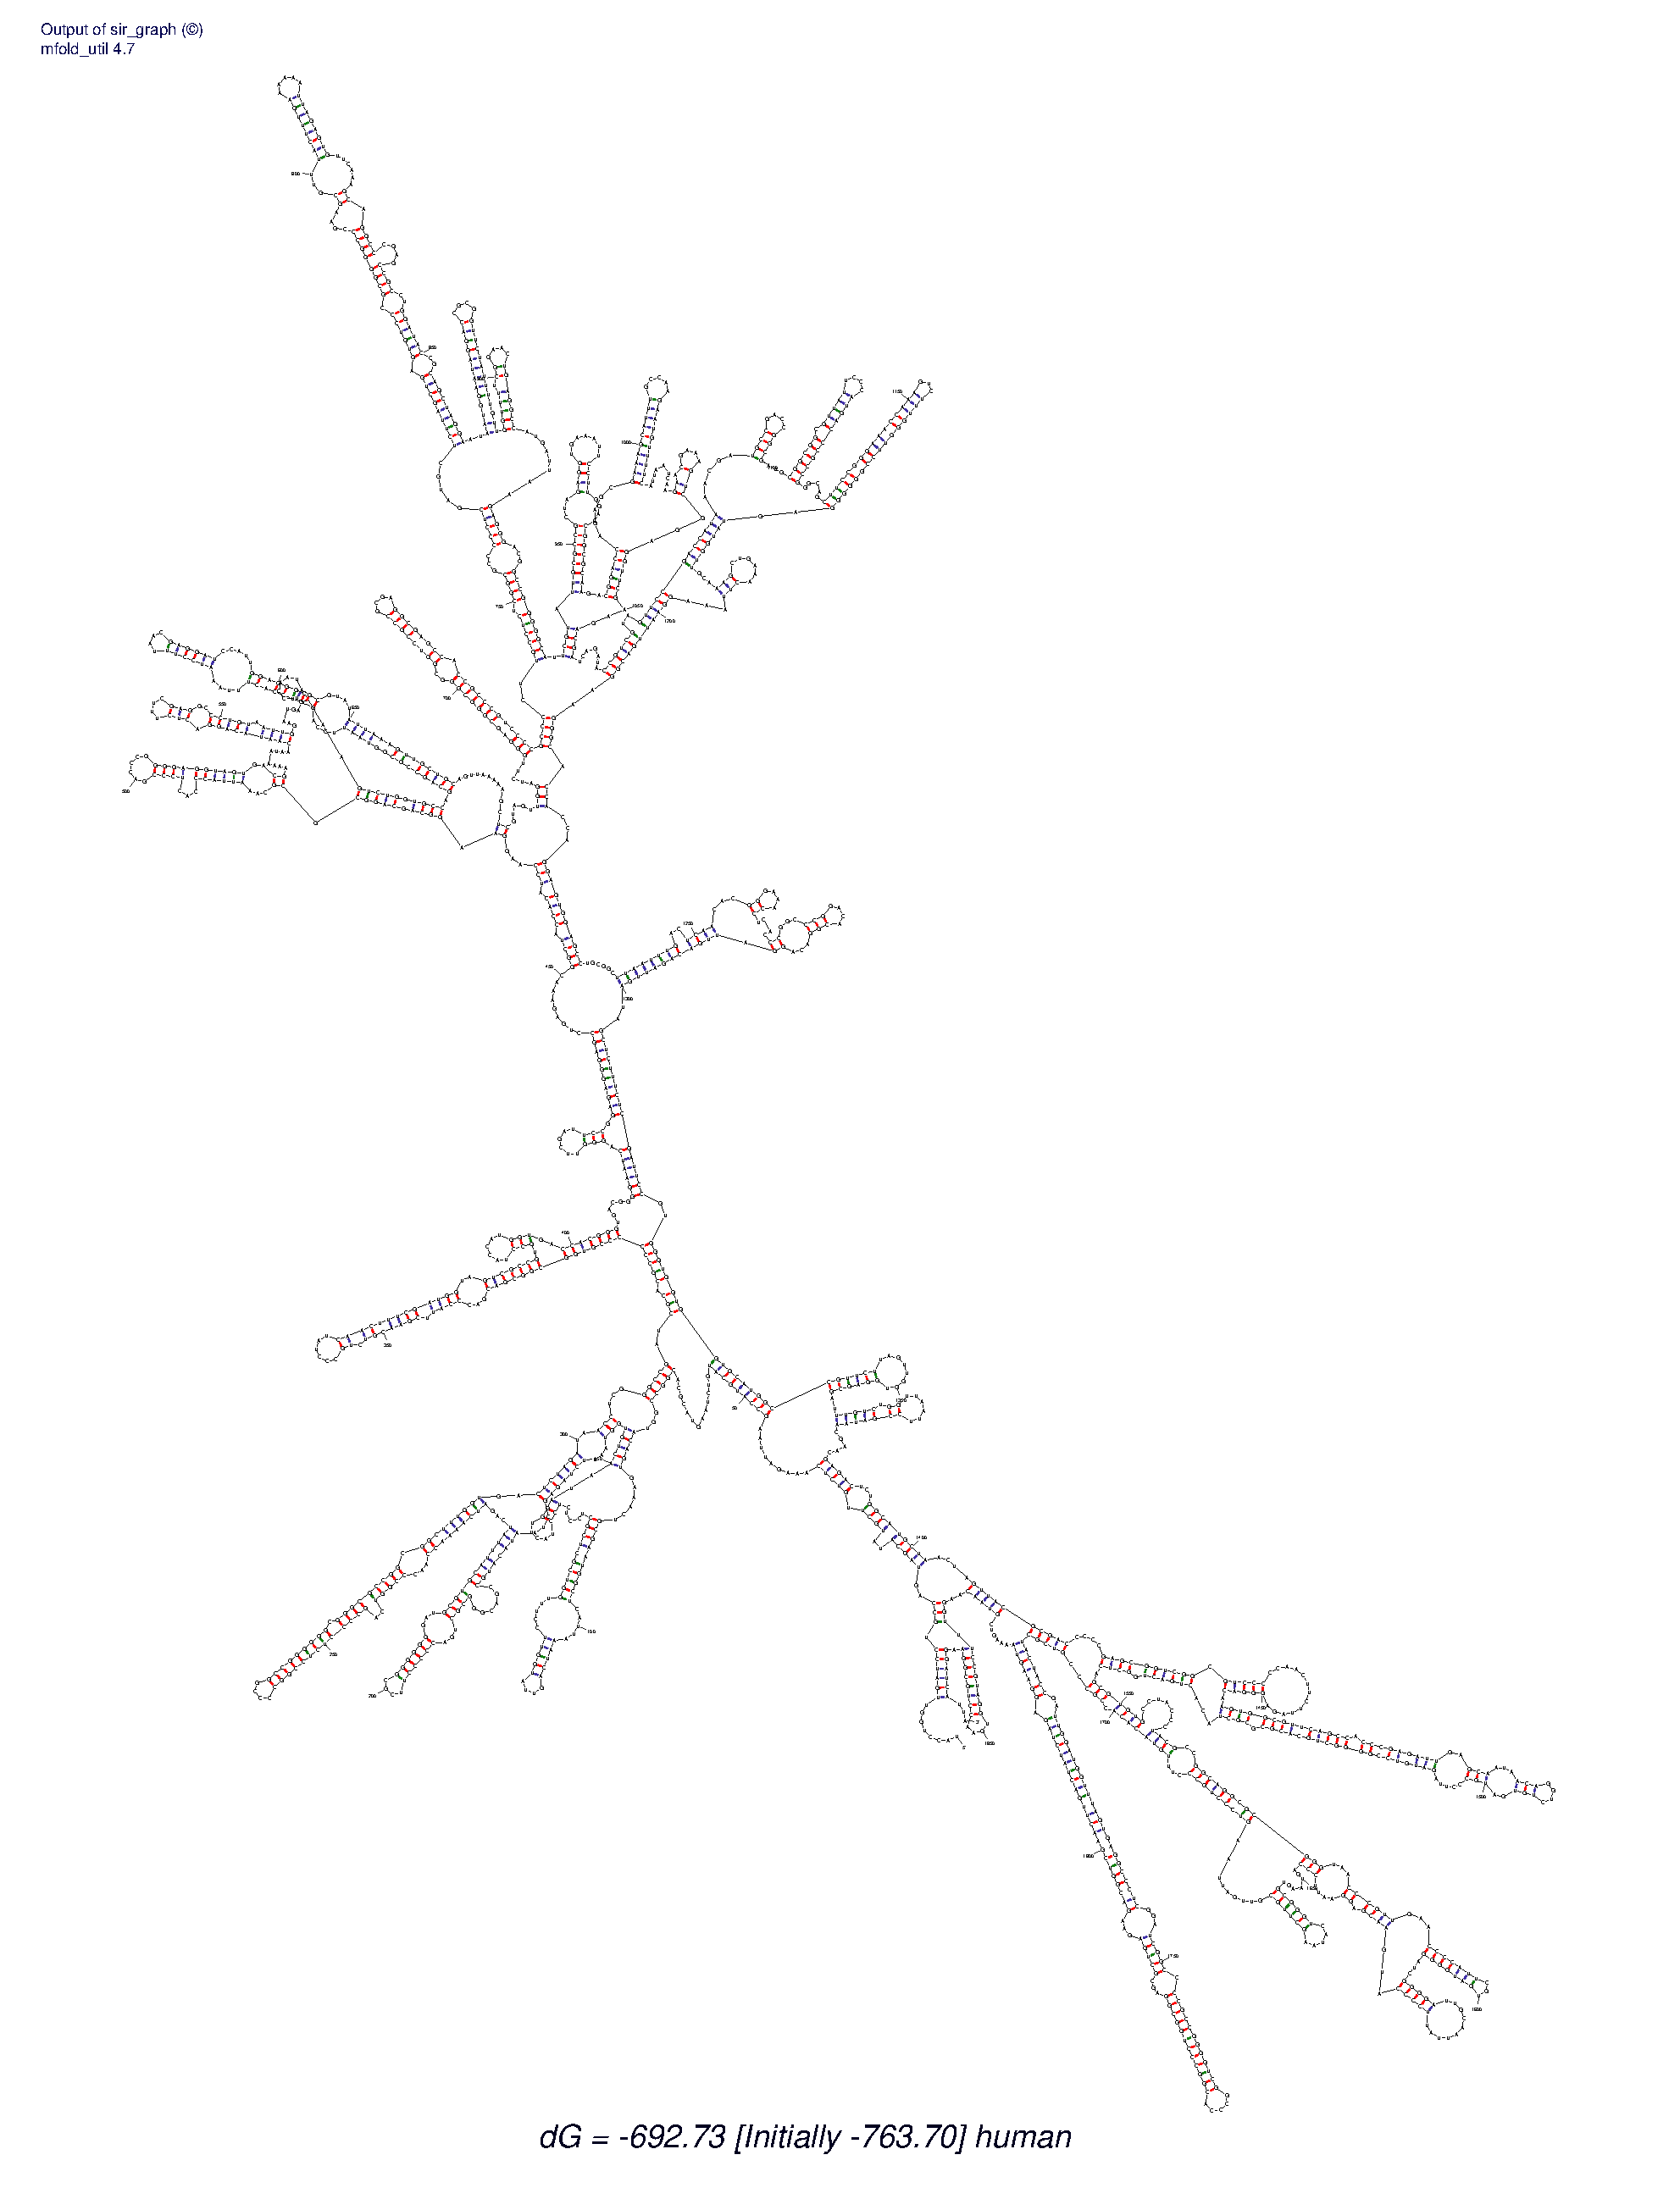
\includegraphics[trim=0 0 2cm 0, width=1\textwidth]{../img/human_mfold}
  \caption{Malá podjednotka vygenerovaná programom Mfold \citenum{MFOLD}}
  \label{obr:RNA_human_mfold}
\end{figure}

\begin{figure}
%trim=left bottom right top
  \centering
  \includegraphics[clip, trim=2.5cm 10cm 3cm 10cm, angle=90, width=1\textwidth]{../img/human_RNAfold}
  \caption{Malá podjednotka vygenerovaná programom RNAfold \citenum{VIENNA_RNA}}
  \label{obr:RNA_human_rnafold}
\end{figure}

Ribozomálnu RNA sme zvolili kvôli jej konzervovanosti naprieč evolučným spektrom. Ďalším
dôvodom bola jej veľkosť, ktorá robí existujúcim nástrojom najväčšie problémy
pri vizualizácií. Na obrázku \ref{obr:RNA_human_crw} vidíme sekundárnu štruktúru 
K03432 malej podjednotky ribozomálnej RNA človeka z CRW databázy.
Tá znázorňuje predstavy biológov o tom, ako by malo nakreslenie danej molekuly vyzerať.
Obrázky \ref{obr:RNA_human_mfold} a \ref{obr:RNA_human_rnafold} sú zase vygenerované
vizualizácie pomocou programov Mfold a RNAfold.
Dodržiavanie základných kritérií ako rovinnosť, loopy na kružniciach a stemy na priamkach
sa viac, či menej programom darí, no celkový vzhľad obrázkov je úplne odlišný od požiadavok
biológov, keďže sa motívy z obrázka z CRW databázy hľadajú veľmi ťažko.


\section{Grafové pojmy}

Potrebujeme si definovať značenie a pojmy, ktoré budeme používať naprieč celou prácou.
Z väčšej časti použijeme značenie od \citet{RTED}.

\subsection{Značenie}

\begin{definice}\label{def:strom}
  Usporiadaný zakorenený strom je orientovaný graf, v ktorom platí, že v ňom neexistujú cykly
  a že hrany sú orientované vždy v smere z predka na potomka.
  Okrem koreňa má každý vrchol svojho predka. Naviac tu existuje usporiadanie medzi potomkami.
  \\
  Usporiadany les je usporiadaná množina stromov.
  %TODO: obrázok usporiadania stromov
\end{definice}

Ak \tree{F} je les, $V_F$ budeme označovať množinu jeho vrcholov a $E_F$ množinu jeho hrán.
Prázdny strom/les budeme značiť $\emptyset$.

Podles lesa \tree{F} je les \tree{G} s vrcholmi $V_{\tree{G}} \subseteq V_{\tree{F}}$
a hranami $E_{\tree{G}} \subseteq E_{\tree{F}} \cap (V_{\tree{G}} \times V_{\tree{G}})$.
Obdobne to plati aj pre podstrom stromu.

Nech $v$ je vrchol stromu \tree{F}. Potom \tree{F_{v}} budeme značiť podstrom \tree{F} zakorenený vo $v$,
t.j. v strome ostávajú iba potomkovia $v$.
\\
\tree{F - v} budeme značiť les, ktorý vznikne zmazaním vrcholu $v$ z \tree{F} spolu so
všetkými hranami obsahujúcimi $v$. Podobne \tree{F - \tree{F_{v}}} budeme značiť les, ktorý
dostaneme zmazaním podstromu \tree{F_{v}} z \tree{F}.

\begin{definice}
  Nech \tree{F} je strom, $u$ a $v$ jeho dva rôzne vrcholy.
  Hovoríme, že $u$ je predkom $v$ ($v$ je potomok $u$) ak $(u, v) \in E_{\tree{F}}$.
  Hovoríme, že $u$ je súrodencom $v$, ak sú to rôzne vrcholy a majú spoločného predka.
\end{definice}



\section{Stromová reprezentacia sekundarnej struktury}

Definicia \ref{def:RNA_sekundarna_struktura} nám ponúka reprezentovať sekundárnu štrukturu
ako usporiadaný strom.

\begin{figure}[H]
\centering
%TODO: vlastny obrazok... namiesto clankoveho
\includegraphics[width=130mm, height=70mm]{../img/stromova_reprezentacia_rna.png}
\caption{Varianty reprezentacie vrcholov}
\label{obr:RNA_vrcholy}
\end{figure}

Bez ujmy na obecnosti budeme o RNA hovoriť ako o strome, aj keď sa môže stať, že
štruktúra nebude celistvá (teda nieje to strom, ale les). V tom prípade ale
iba pripojíme koreňový vrchol, ktorého potomkovia budú dané stromy.

Každý vrchol stromu môže reprezentovať napríklad motiv v štruktúre RNA, nukleotid, alebo bázovy pár
Príklady možno vidiet na obrázku \ref{obr:RNA_vrcholy}.

V našej práci vrchol stromu reprezentuje bázovy pár (vnútorný vrchol) a nespárovanú bázu (list stromu).
Štruktúru, do ktorej patrí si totiž vieme ľahko zistiť z potomkov vrcholu.


\input{rna_to_tree}



